\documentclass[12pt]{article}

\usepackage[utf8]{inputenc}%encodage des caractères
\usepackage[T1]{fontenc}%encodage de la police
\usepackage[french]{babel}%langue française
\usepackage{graphicx}
\usepackage{amsmath}

\begin{document}

\begin{titlepage}

\title{Rapport du projet Conception logicielle avancée\\\bigskip
Sujet : Éditeur de livres dont vous êtes le héros}
\author{Dorlodot Des Essarts, Duclos, Guillot, Lebreton, Longuet}
\date{05 avril 2022}
\maketitle
\begin{figure}[htp]
  
  \centering
    
\includegraphics[width=0.5\textwidth]{Logo_unicaen}
\end{figure}
\vfill
\vfill
\begin{flushleft}
Encadrants :\\
M. Grégory Bonnet\\
M. Meddouri Nida\\
\bigskip
Année : 2021-2022\\
\end{flushleft}

\hfill
\thispagestyle{empty}
\setcounter{page}{0}
\end{titlepage}

\tableofcontents

\newpage
	
\section{Introduction}
\subsection{Description du sujet de projet}
Énoncé : Les livres dont vous êtes le héros (ou LDVEH) sont des jeux de rôles en solitaire dont la
narration est décomposées en paragraphes, dispersés dans le livre. Des liens, en fonction des choix
du lecteurs, permettent de naviguer d’un paragraphe à l’autre.\medskip
\\
Dans un premier temps, il s’agira de développer un éditeur de texte qui maintienne le graphe du jeu 
et qui puisse réorganiser aléatoirement le livre. L’affichage de la ou les solutions (paragraphe devant être traversés pour
gagner) devront être calculées ainsi que la difficulté du jeu (proportions de solutions au regard des
chemins possibles).\medskip
\\
Dans un second temps, il s’agira d’ajouter un système de rencontres et de combat, ainsi que la gestion d’objets ou d’indices qui peuvent être nécessaire pour gagner. \medskip
\\
Enfin, un mode lecture permettant de jouer au LDVEH pourra être implanté.

\subsection{Présentation du plan du rapport}
Nous allons décomposer le rapport de la façon suivante, une première partie explicative sur notre interprétation du projet et des travaux existants sur l'internet.\\
Puis, la décomposition fonctionnelle de notre programme et la répartition du travail au sein de notre groupe.\\
Et enfin, le détail des algorithmes utilisés, le détail des méthodes présentes dans notre programme et les résultats obtenus.


\newpage
\section{Objectif du projet}
\subsection{Interprétation du sujet de projet}
Nous avons choisi de réaliser dans un premier temps un éditeur d'histoire en console, puis de proposer une alternative avec une interface graphique.\\
Pour cela nous devions apprendre à manipuler les fichiers sur un système d'exploitation, la création de menu dans la console en langage Java.\\
Et au fur et à mesure de notre avancement, d'ajouter des fonctionnalités permettant de rendre l'histoire plus personnalisable.
\subsection{Description de travaux existants sur le même sujet	}

Dans le cahier des charges nous avions des exemples afin de bien comprendre le système du "livre dont on est le héros".\\
Ce premier lien, nous permet de visualiser les fonctionnalités implémentées dans le logiciel afin de aiguiller sur des mécanismes de programmation pertinentes et intéressantes pour notre projet.\medskip
\\
http://litteraction.fr/presentation/livre-dont-on-est-le-heros/logiciels \medskip
\\
Le deuxième lien permet de tester un logiciel fonctionnel et disponible librement en ligne, réalisé cependant en langage JavaScript. Ce logiciel nous permet de visualiser le rendu final en mode lecture d'une histoire.\medskip
\\
https://projectaon.org/staff/christian/gamebook.js/

\begin{figure}[htp]
  
  \centering
    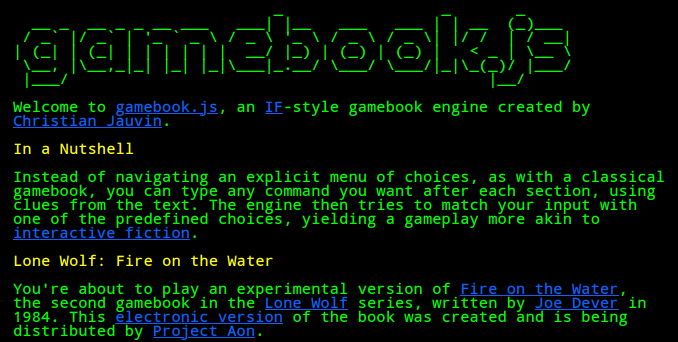
\includegraphics[width=0.8\textwidth]{Exemple}
\end{figure}

\newpage
\section{Fonctionnalités implémentées}
\subsection{Description des fonctionnalités}
\noindent
Voici les fonctionnalités disponibles dans notre programme :\bigskip
\\
-Un mode d'emploi de notre éditeur d'histoire pour une rapide compréhension de celui-ci.
\\
-Textes et règles de l'histoire personnalisables par l'utilisateur.\\
Afin d'indiquer à la personne qui va jouer l'histoire les fonctionnalités à sa disposition.\medskip
\\
-Personnaliser l'arbre du déroulement de l'histoire (nombre de branches, de nœuds...).\\
La possibilité d'ajouter ou d'enlever des nœuds afin de modifier la difficulté de l'histoire.\medskip
\\
-Implémentation de l'inventaire du joueur.\medskip
\\
-Un mode lecture pour l'histoire créée.\\
Pour directement jouer l'histoire par un utilisateur.\medskip
\\
-Interface console afin de visualiser le déroulement du programme.\medskip
\\
-Création du graphique représentatif de l'histoire, les différents choix que le créateur de l'histoire a implémenté.
\subsection{Organisation du projet}
Pour la répartition du travail, nous nous sommes répartis différentes parties essentielles du programme.\\
Nous avons été rejoint par Arthur Dorlodot Des Essarts après les vacances d'hiver.\medskip
\\
\clearpage
Arthur Dorlodot Des Essarts a directement commencé l'interface graphique de l'étideur d'histoire avec Java Swing.\\
Alexandre Duclos a  travaillé sur la gestion des fichiers textes (la création, l'édition, etc), la réalisation du rapport.\\
Benjamin Guillot quant à lui a réalisé les contrats de chaque méthodes de nos programmes, la génération de la Javadoc.\\
Nohan Lebreton,création de l'inventaire et du main du projet, puis a rejoint Arthur Dorlodot Des Essarts sur l'interface graphique sur JTree puis sur Swing.\\
La réalisation de l'éditeur console et de la conception de l'architecture afin de créer une histoire personnalisable facilement a été faite par Brian Longuet.

\begin{figure}[h]
  \centering
    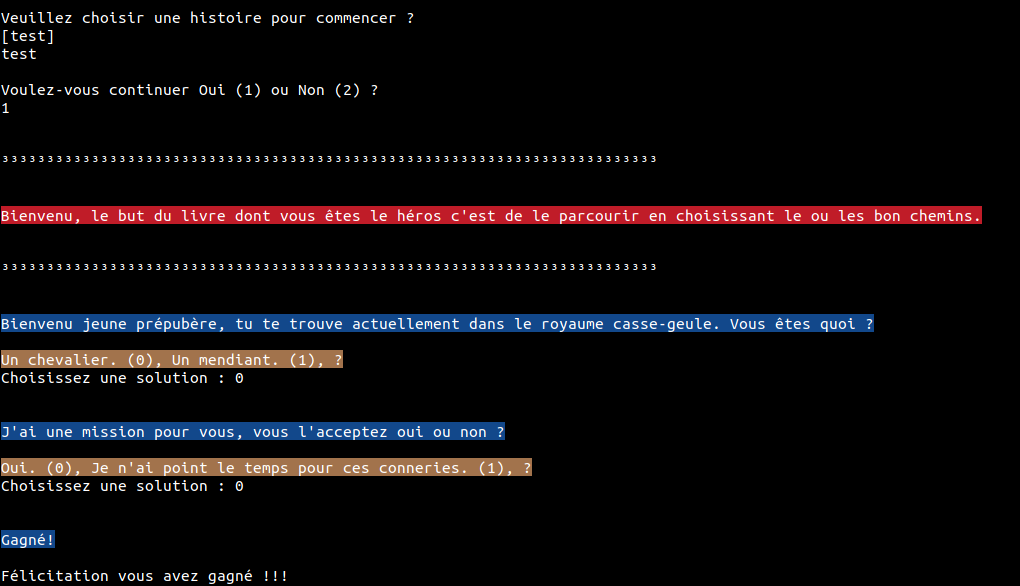
\includegraphics[width=1\textwidth]{Test}
\end{figure}
\clearpage
\section{\'Elements techniques}
\subsection{Description des paquetages non standards utilisés}
Nous avons utilisé JTree puis Java Swing afin de réalisé notre interface graphique que nous avons appris durant ce semestre en Complément Programmation Orienté Objet mais par manque de temps nous n'avons pas terminé l'implémentation de nos programmes dans celle-ci.


\subsection{Description des algorithmes}
\noindent
-Gestion des fichiers : \\
\indent
Création des fichiers dans un dossier spécifique\\
\indent
Possibilité de modifier, supprimer, déplacer les fichiers\\
\indent
Accéder et lire les fichiers\\
-Gestion des étages :\\
\indent
	Création de nœuds\\
\indent
	L'affichage des textes de l'histoire \\
-Gestion du graphique :\\
\indent	
	Génération du graphique de l'histoire avec les solutions\\
\indent	
	Affichage de celui-ci grâce au menu console\\
-Gestion de l'interface console :\\
\indent	
	Création du menu de navigation\\
\indent	
	Ajout de couleurs afin d'améliorer la lisibilité\\

\clearpage
\section{Architecture du projet}
\subsection{Diagrammes des modules et des classes}
Voici l'arborescence de notre dossier de projet en 2 captures :
\begin{figure}[h]
  \centering
    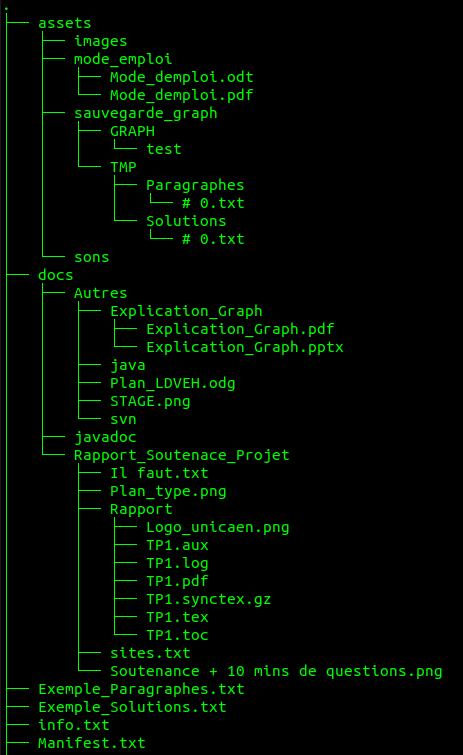
\includegraphics[width=0.6\textwidth]{Tree1}
    
\end{figure}
\clearpage
\begin{figure}[h]
  \centering
    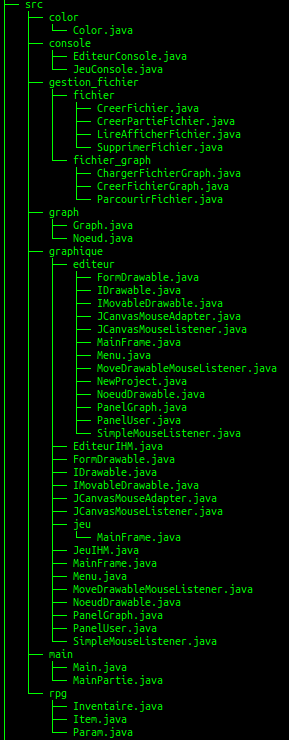
\includegraphics[width=0.6\textwidth]{Tree2}
\end{figure}


\clearpage
\section{Expérimentations et usages}
\subsection{Cas d'utilisation}
Nous disposons d'un mode d'emploi en pdf dans le dossier du projet afin d'expliquer les différentes fonctionnalités de notre programme.\medskip
\\
\noindent
Nous obtenons ce menu lors de l'exécution du programme, et l'arborescence créée par le programme :
\begin{figure}[h]
  \centering
    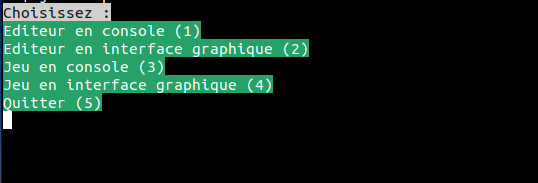
\includegraphics[width=0.8\textwidth]{Menu}
    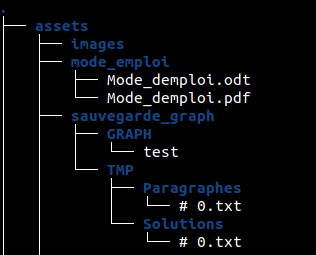
\includegraphics[width=0.8\textwidth]{Tree3}
\end{figure}

\clearpage
\subsection{Résultats quantifiables}
On obtient la génération du graphique en console sur le première capture, ou encore ce resultat lors de la sauvegarde de l'histoire afin de pouvoir l'éditer plus tard, sur la deuxième capture :\\
\begin{figure}[h]
  \centering
    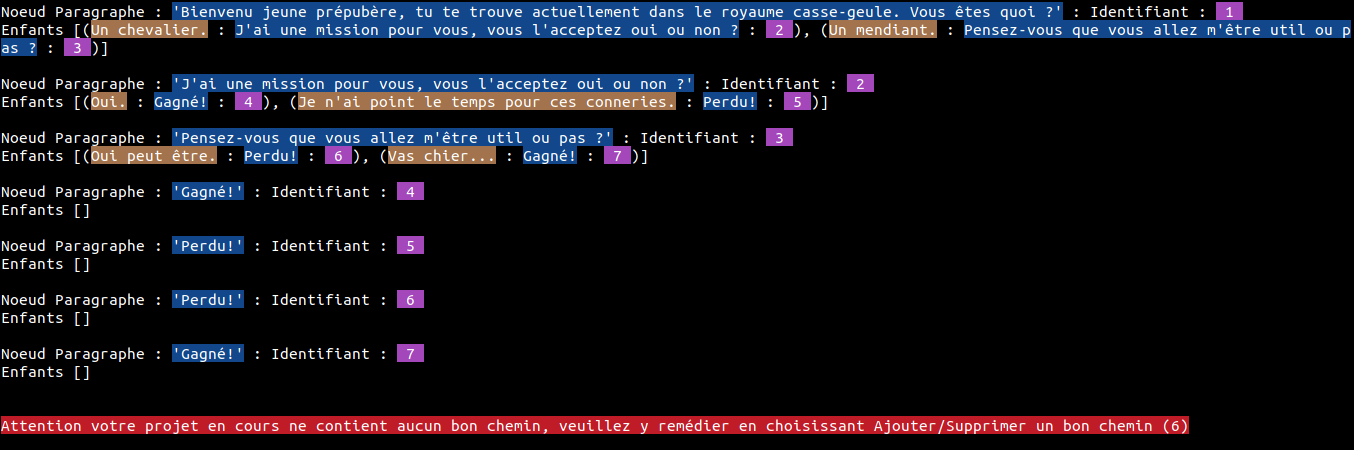
\includegraphics[width=1\textwidth]{Graph}
\end{figure}

\begin{figure}[h]
  \centering
    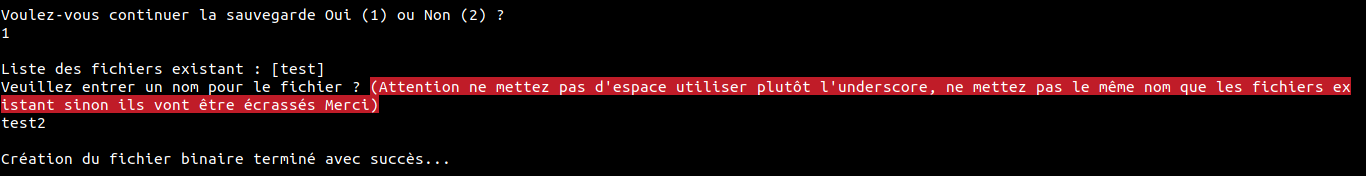
\includegraphics[width=1\textwidth]{Save}
\end{figure}

\clearpage
\section{Conclusion}
Ce projet nous a permis de concevoir un éditeur "d'histoire dont vous êtes le héros" avec le langage Java.
Au cours de ce stage, nous avons réinvesti et mis en pratique, de nombreuses notions de programmation orientée objet, abordées au
semestre de licence 2 informatique. De plus, nous avons exploité de nouvelles possibilités de réalisation de projet avec l'utilisation de la forge SVN de l'université de Caen.\\
Pour conclure, ce projet était très intéressant à plus d’un titre. En effet, la conception d'un programme pouvant modifier spécifiquement des fichiers créés par ce même programme, d'offrir la possibilité de façonner l'histoire créée autant que l'utilisateur le souhaite était instructif.\bigskip
\\
\\
Nous avions comme perspectives d'amélioration, d'une part une interface graphique avec des zones de textes, des boutons, etc afin d'avoir une alternative à l'interface par console que nous avons actuellement mais par manque de temps elle n'a pas pu être finalisée.\\
D'autre part, un graphique final de l'histoire créée dans une fenêtre ayant la possibilité de modifier chaque paramètre, comme les textes de chaque nœud, ajouter ou supprimer des partie de l'histoire.\\
L'ajout de sons et d'images pour certaines actions, le début de l'histoire en mode lecture, le fait de gagner ou de perdre.

\end{document} 